\documentclass[a4paper]{report}

% --- Configurações Básicas ---
\usepackage[T1]{fontenc}      % Codificação de saída da fonte (Importante!)
\usepackage[utf8]{inputenc}   % CORREÇÃO: É 'utf8' (sem hífen)
\usepackage[english]{babel}   % Idioma do documento (para hifenização correta)
\usepackage{float} % Opcional, mas recomendo MUITO (explico abaixo)
\usepackage[margin=1in]{geometry}
\usepackage{graphicx}
\usepackage{amsmath}
\usepackage{setspace}
\usepackage[table,xcdraw]{xcolor}
\usepackage[hidelinks]{hyperref}
\usepackage{fancyhdr}
\usepackage{tocloft}
\usepackage{booktabs}   
\usepackage{parskip}          % DICA: Remove indentação e adiciona espaço entre parágrafos (comum em manuais de engenharia)

% --- Metadados ---
\title{Steering Effort Calculation and Validation Handbook}
\author{Vinicius Andrade Trento}
\date{\today}
\onehalfspacing


% --- Cabeçalho e Rodapé ---
% \pagestyle{fancy}
% \fancyhf{} % Limpa configurações padrão
% \fancyhead[L]{Steering Effort Handbook}
% \fancyhead[R]{Vinicius Trento - PUCPR Racing}
% \fancyfoot[C]{\thepage} % Numeração de página no centro do rodapé


\begin{document}

\maketitle

\tableofcontents
\vspace{4cm}
% O comando \newpage não é estritamente necessário aqui pois \chapter já quebra página, 
% mas não faz mal mantê-lo se quiser garantir uma página em branco extra.

\begin{figure}[H] 
    \centering
    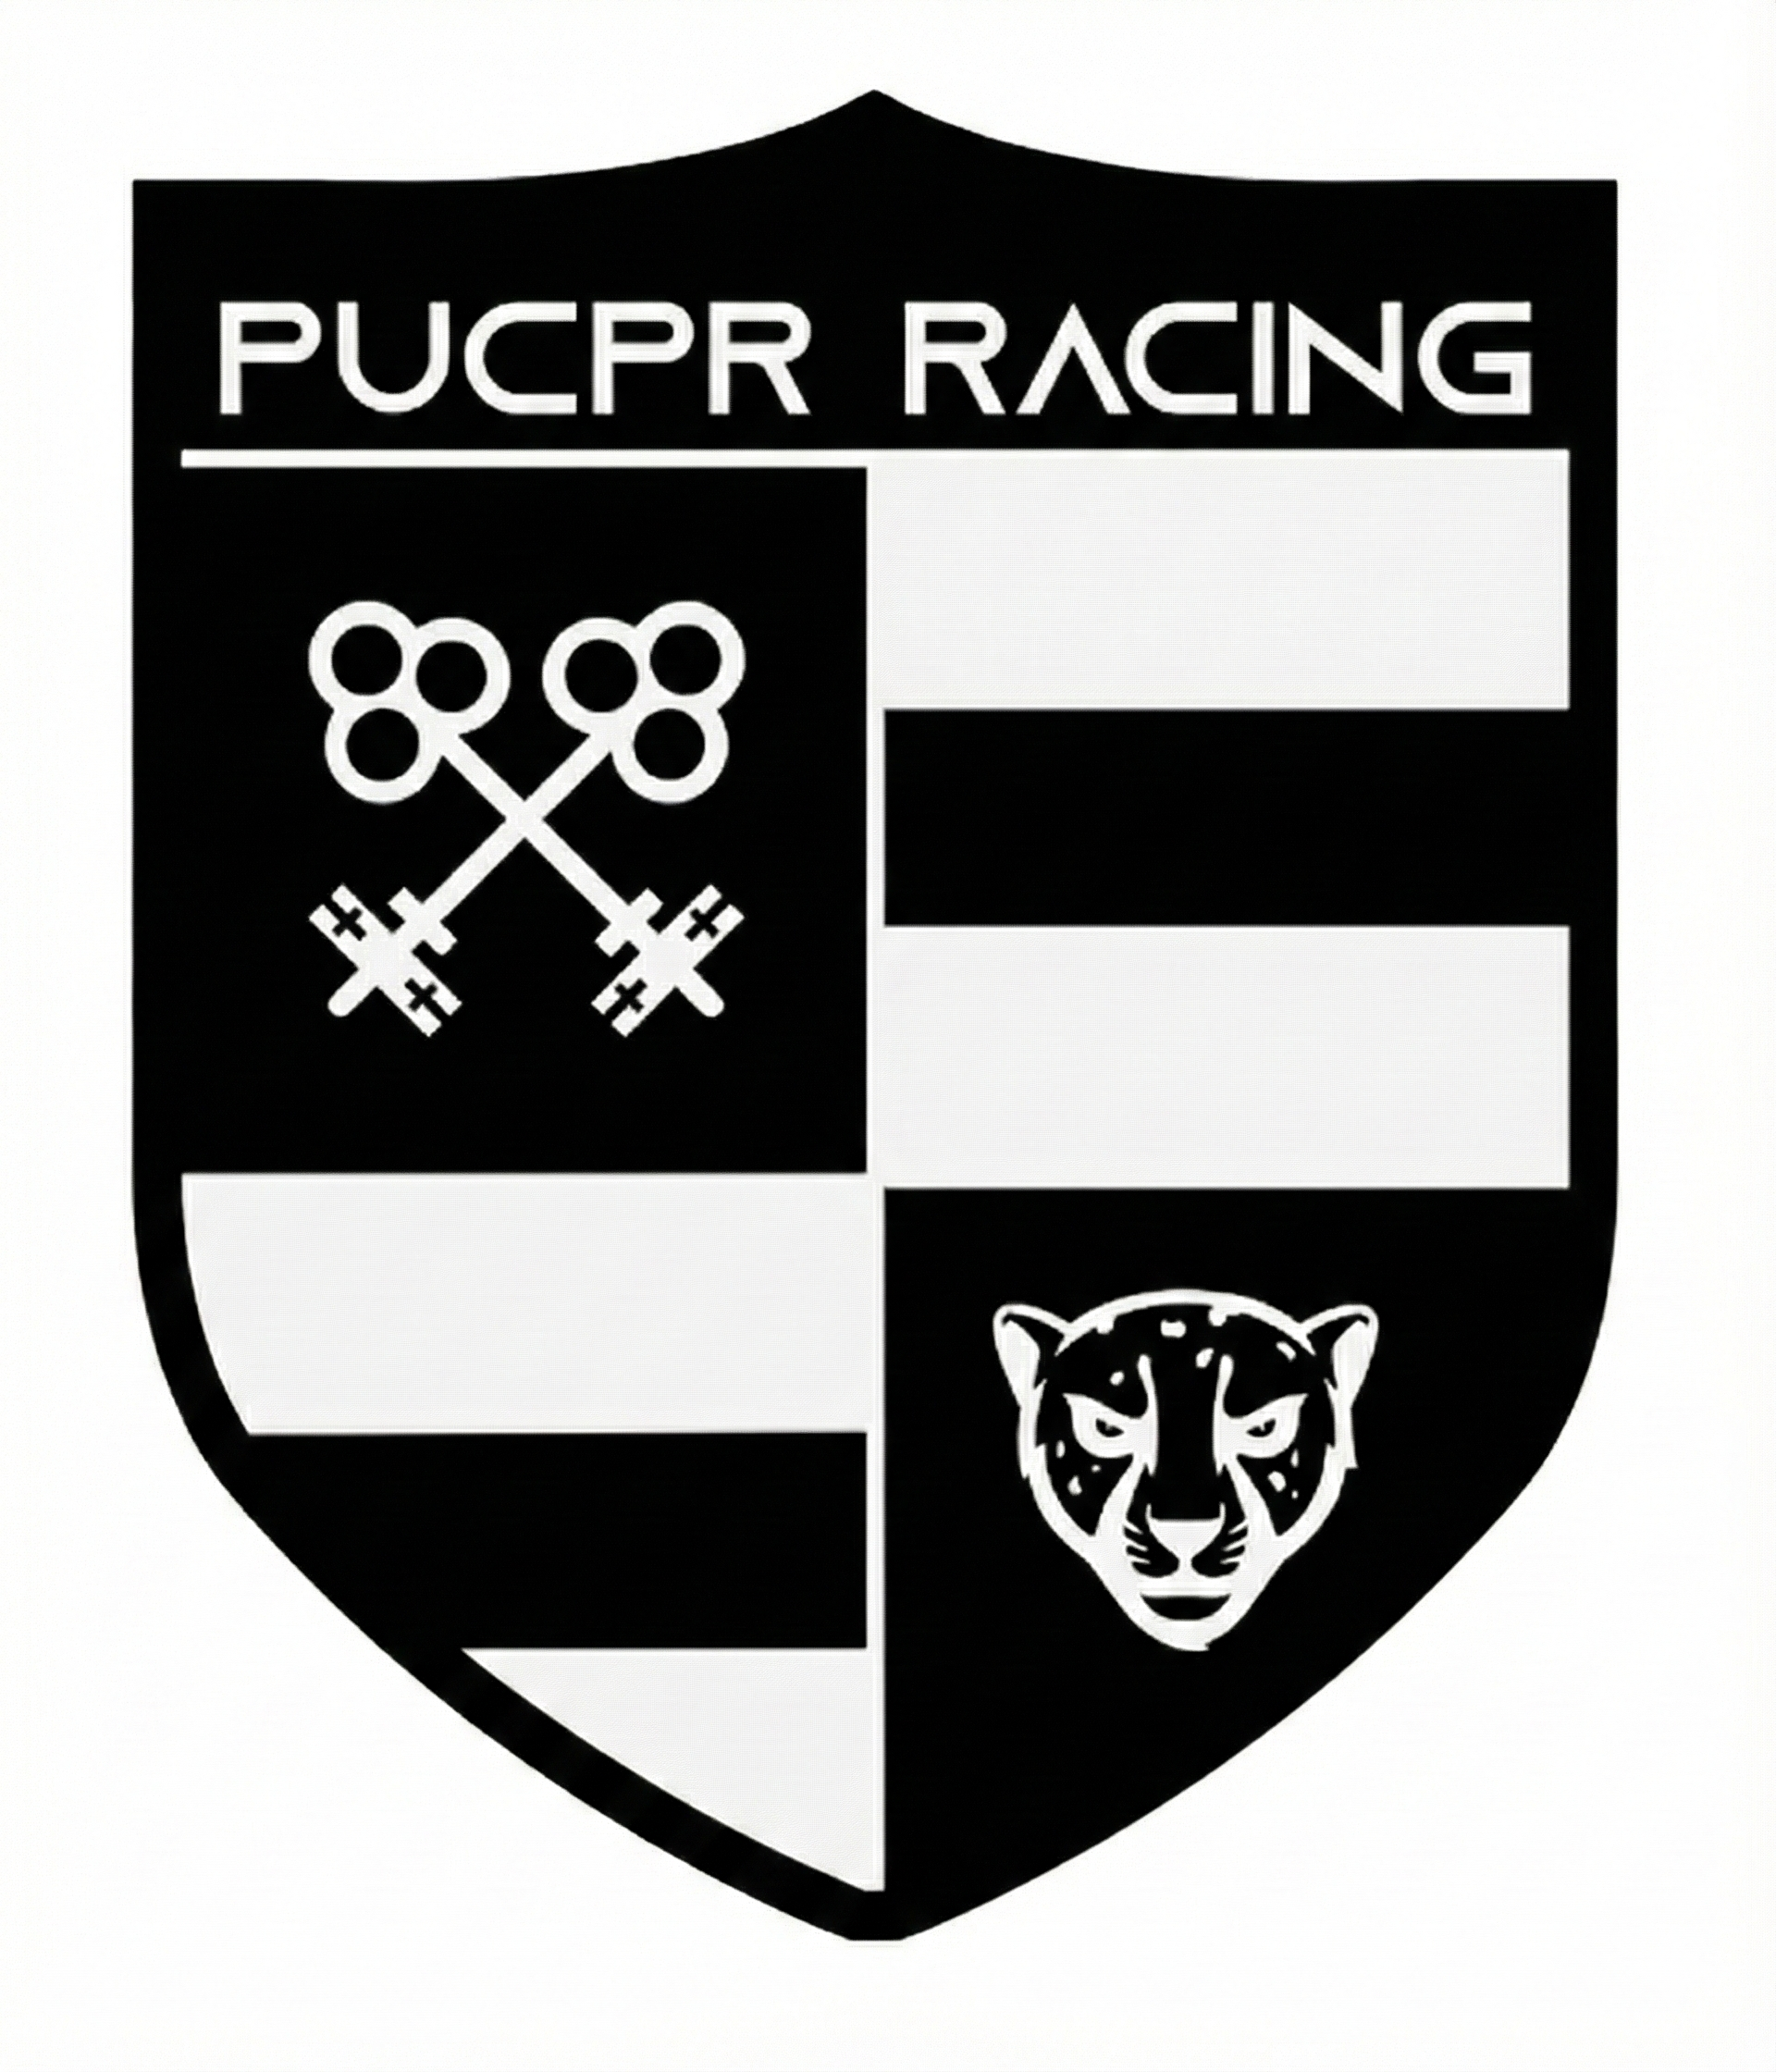
\includegraphics[width=0.3\textwidth]{Images/logo_equipe.png}
    % \caption{a}
\end{figure}

\chapter{Introduction}
\section{Purpose}
This handbook documents the steering effort calculation and validation procedures for the FSAE26 vehicle. It provides comprehensive guidelines for analyzing steering system performance and ensuring design requirements are met.

As explained by Pfeffer and Harrer \cite{Lenkungshandbuch}, the steering system's performance is critical for vehicle handling and driver comfort, playing a crucial role in lateral dynamics. 


\section{Scope}

\begin{itemize}
    \item Steering system analysis methodology
    \item Calculation procedures and formulas
    \item Validation testing protocols
    \item Performance benchmarks
\end{itemize}

\section{Methodology}
The steering effort is calculated based on vehicle dynamics principles, considering factors such as tire forces, steering geometry, and driver input. Validation is performed through controlled testing to compare calculated values with real-world measurements. 

\chapter{Steering System Overview}
\section{System Components}

The steering system consists of the following key components:

\begin{itemize}
    \item Steering Wheel
    \item Steering Column
    \item Rack and Pinion
    \item Tie Rods
\end{itemize}

Well represented in the literature, these components work together to translate driver input into wheel movement, affecting vehicle direction and handling characteristics.

Below follows a schematic representation of the steering system components and their usual assembly in a typical FSAE vehicle.

\vspace{0.5cm}

\begin{figure}[H] 
    \centering
    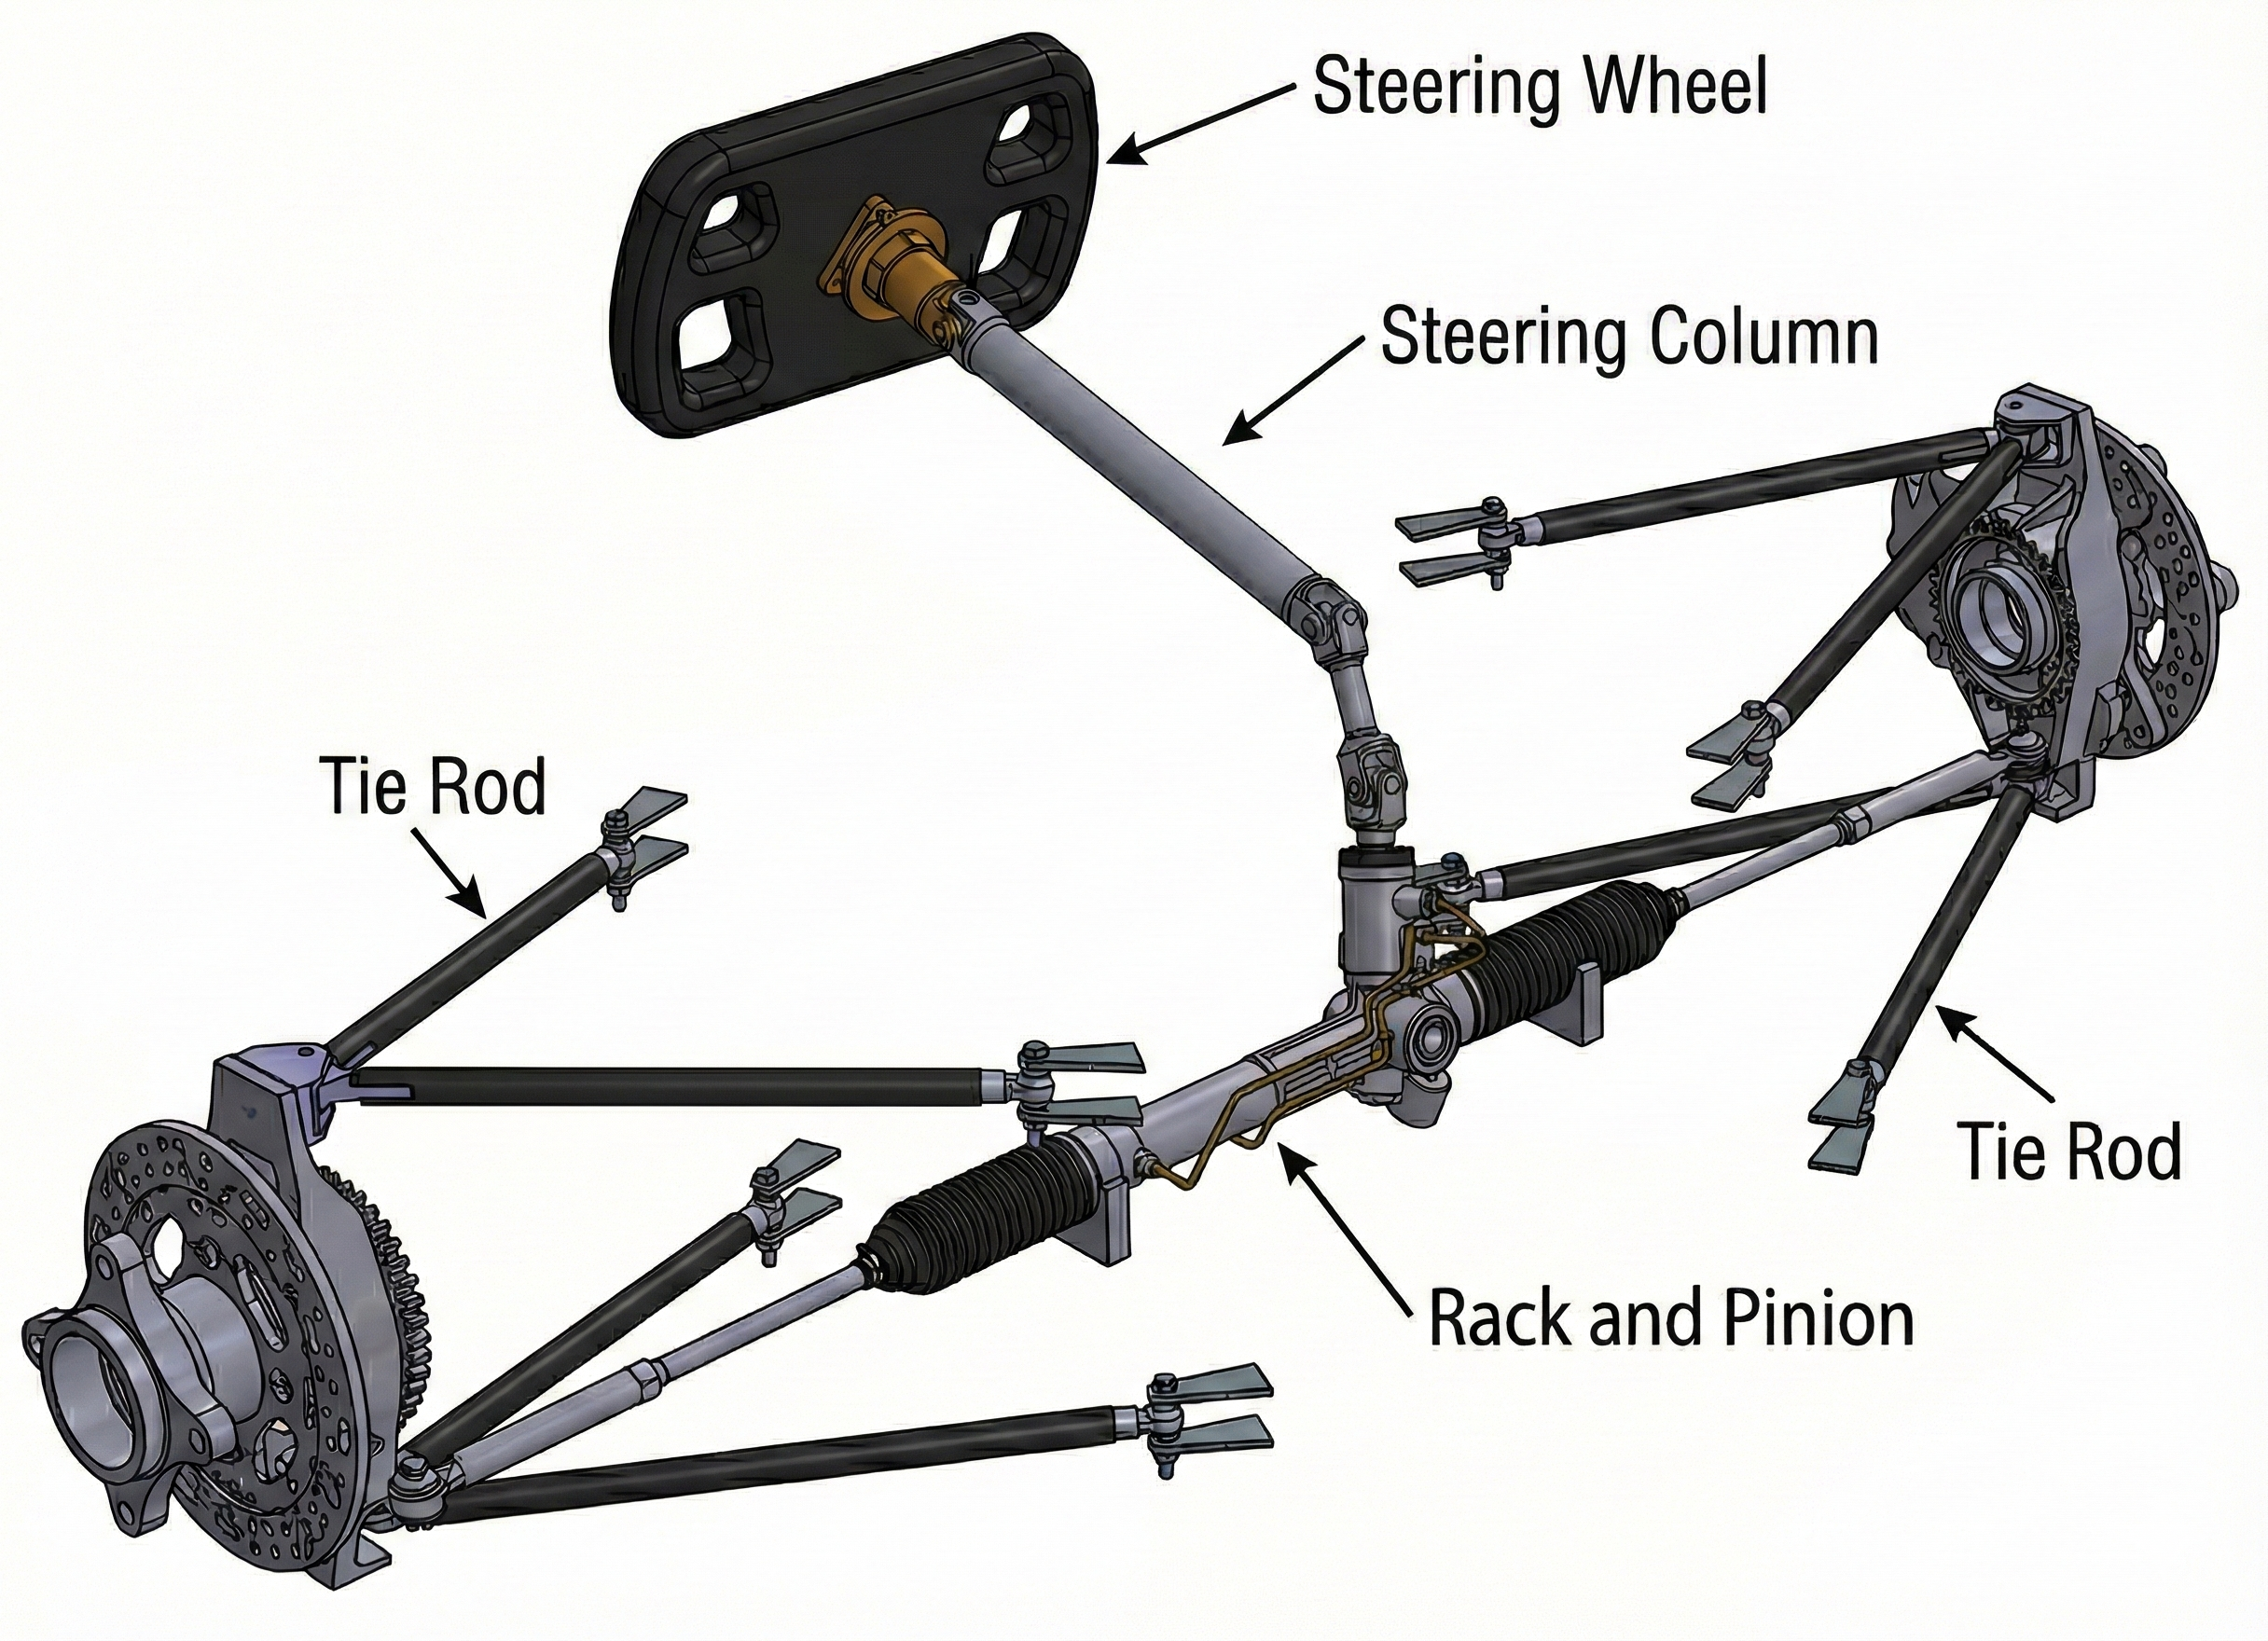
\includegraphics[width=0.6\textwidth]{Images/steering_system.png}
    \caption{Steering System Components}
\end{figure}

\section{Design Requirements}
A good steering system must meet the following design requirements:

\begin{itemize}
    \item Provide adequate feedback to the driver
    \item Minimize steering effort
    \item Ensure precise control and responsiveness
    \item Maintain durability under racing conditions
    \item Avoid compliance issues between suspension components  
\end{itemize}

Thus in order to be able to track these requirements, the steering effort calculation and validation is of utmost importance. 

The first step will be deciding targets for the main indicatior, the steering effort. Based on previous years' data and literature review ~\cite{Lenkungshandbuch}, a target steering effort of 15 Nm at 1g lateral acceleration is set for the FSAE26 vehicle.  

\chapter{Calculation Methodology}

The computational model developed for this study utilizes a deterministic approach based on Rigid Body Mechanics, implemented via a Python script. The algorithm evaluates the steering torque requirements by decomposing the forces at the contact patch and transposing them to the steering wheel through the kinematic chain. The analysis is bifurcated into two distinct operational domains: Static Steering (Parking) and Dynamic Cornering.

\section{Theory and Formulas}

\subsection{Geometric and Kinematic Definitions}

Before calculating forces, the model establishes the kinematic relationship between the driver's input and the wheel's reaction using the Steering Ratio (Kinematische Lenkübersetzung). The total ratio ($i_S$) is derived from the rack-and-pinion geometry:

\begin{equation}
    i_S = \frac{L_{steering\_arm}}{r_{pinion}} 
    \label{eq:Steering_Ratio}
\end{equation}

Additionally, the Mechanical Trail (Nachlaufstrecke) is computed as a function of the dynamic wheel radius ($R_{dyn}$) and the Caster angle ($\nu$):

\begin{equation}
    t_{mech} = R_{dyn} \cdot \tan(\nu)
    \label{eq:Mechanical_Trail}
\end{equation}

\subsection{Static Steering Scenario (Standlenken)}
In the condition where lateral acceleration is zero ($a_y = 0$), the primary resistive load is the friction generated by twisting the stationary tire contact patch.
\begin{itemize}
    \item Tire Contact Patch Estimation: The model assumes a circular contact patch geometry. The area is derived from the vertical wheel load ($F_Z$) and the tire inflation pressure ($p_{tire}$), allowing for the calculation of an equivalent patch radius ($r_{p}$):
    \begin{equation}
        r_{p} = \sqrt{\frac{F_Z / p_{tire}}{\pi}}
        \label{eq:Tire_Patch}
    \end{equation}
    
    \item Scrub Torque (Bohrmoment): The resistive moment caused by the friction of the tire rubber on the asphalt is calculated using a integration approximation for a uniform pressure distribution:
    
    \begin{equation}
        M_{scrub} = \frac{2}{3} \cdot \mu_{static} \cdot F_Z \cdot r_{p}
        \label{eq:Scrub_Torque}
    \end{equation}
    Where $\mu_{static}$ is the coefficient of static friction.

\end{itemize}

\subsection{Dynamic Cornering Scenario (Fahren in der Kurve)}

When the vehicle is in motion ($a_y > 0$), the resistive load shifts from dry friction to the forces generated by the tire's slip angle. Self-Aligning Torque $M_{SAT}$ (Rückstellmoment aus Seitenkraft):

\begin{itemize}
    \item The model calculates the lateral force ($F_{lat}$) acting on the front axle based on the vehicle mass and lateral acceleration. The resulting torque is the product of this force and the total ground trail (sum of mechanical and pneumatic trail):
    \begin{equation}
        M_{SAT} = F_{lat} \cdot (t_{mech} + t_{pneu})
        \label{eq:Self_Aligning_Torque}
    \end{equation}
\end{itemize}

\subsection{Geometric Restoring Moment (Gewichtsrückstellung)}

In both static and dynamic scenarios, the model accounts for the Jacking Effect. This is the restoring moment generated because the steering geometry (Caster and Kingpin Inclination) physically lifts the vehicle's chassis during a turn. The script quantifies this as a function of the vertical load ($F_Z$) and the steering angle ($\delta$):

\begin{equation}
    M_{jacking} = F_Z \cdot [r_{scrub} \cdot \tan(\sigma) + t_{mech} \cdot \tan(\nu)] \cdot \sin(\delta)
    \label{eq:Jacking}
\end{equation}

Where $\sigma$ is the KPI angle and $\nu$ is the Caster angle.

\subsection{System Inertia and Final Effort (Lenkradmoment)}

To ensure the model accounts for the haptic feedback during rapid transients, the Effective Inertia (Reduziertes Massenträgheitsmoment) is calculated. The translational mass of the steering rack ($m_{rack}$) is converted into an equivalent rotational inertia at the pinion shaft and added to the pinion's own inertia:
\begin{equation}
    I_{eff} = I_{pinion} + (m_{rack} \cdot r_{pinion}^2)
    \label{eq:Effective_Inertia}
\end{equation}

\textbf{Final Torque Calculation:} The total torque required at the steering wheel ($T_{SW}$) is the sum of the resistive and restoring moments at the Kingpin, divided by the steering ratio, plus a constant term representing the internal mechanical friction ($T_{friction}$) of the steering gear:
\begin{equation}
    T_{SW} = \left( \frac{2 \cdot (M_{scrub} + M_{jacking})}{i_S} \right) + T_{friction}
    \label{eq:Steering_Torque}
\end{equation}

A good reminder is always to check units consistency throughout the calculations to avoid errors. The developed script includes unit checks at each step to ensure accuracy and focuses in useing the \textbf{International System of Units (SI)}.

\section{Input Parameters}
To initialize the analytical model described in the methodology, specific geometric and inertial properties of the vehicle were defined. These parameters represent the vehicle's "As-Designed" configuration. The input variables are categorized into suspension geometry, steering system properties, and operational boundary conditions.

% --- Tabela 1: Geometria ---
\begin{table}[htbp] 
    \centering
    \caption{Vehicle and Suspension Geometry (Fahrwerkgeometrie)}
    \label{tab:geometry} % Label corrigida
    \renewcommand{\arraystretch}{1.2} 
    
    \begin{tabular}{lccl} 
        \toprule
        \rowcolor[HTML]{EFEFEF} 
        \textbf{Parameter} & \textbf{Symbol} & \textbf{Value [Unit]} & \textbf{Description} \\ 
        \midrule
        Total Vehicle Mass & $m_{total}$ & 376 [kg] & Total mass (Driver + Fluids) \\
        Front Weight Dist. & $W_{front}$ & 50 [\%]  & Static weight distribution \\
        Caster Angle       & $\nu$       & 4.0 [deg] & Nachlaufwinkel (Suspension kinematics) \\
        KPI Angle          & $\sigma$    & 10.0 [deg]& Spreizung (Kingpin Inclination) \\
        Scrub Radius       & $r_{scrub}$ & 35 [mm]  & Lenkrollradius \\
        Dyn. Wheel Radius  & $R_{dyn}$   & 0.23 [m] & Effective radius under load \\
        \bottomrule
    \end{tabular}
\end{table}

% --- Tabela 2: Sistema de Direção ---
\begin{table}[htbp] 
    \centering
    \caption{Steering System Properties (Lenkungsparameter)}
    \label{tab:steering} % Label corrigida para não conflitar com a anterior
    \renewcommand{\arraystretch}{1.2} 
    
    \begin{tabular}{lccl} 
        \toprule
        \rowcolor[HTML]{EFEFEF} 
        \textbf{Parameter} & \textbf{Symbol} & \textbf{Value [Unit]} & \textbf{Description} \\ 
        \midrule
        Pinion Radius  & $r_{pinion}$ & 40 [mm] & Effective radius of the steering pinion gear.\\
        Steering Arm   & $L_{arm}$    & 170 [mm]  & Length of the lever arm at the upright.\\
        Pinion Inertia & $I_{pinion}$ & $6.29 \times 10^{-4}$ [kg$\cdot$m$^{2}$] & Rotational inertia derived from CAD. \\
        Rack Mass      & $m_{rack}$   & 0.587 [kg]  & Translational mass of the rack bar. \\
        System friction& $T_{fric}$   & 4.0 [Nm] & Estimated internal mechanical friction (Reibung). \\
        \bottomrule
    \end{tabular}
\end{table}

% --- Tabela 3: Condições Operacionais (Nova) ---
\begin{table}[htbp] 
    \centering
    \caption{Operational Conditions and Simulation Inputs}
    \label{tab:conditions}
    \renewcommand{\arraystretch}{1.2} 
    
    \begin{tabular}{lccl} 
        \toprule
        \rowcolor[HTML]{EFEFEF} 
        \textbf{Parameter} & \textbf{Symbol} & \textbf{Value [Unit]} & \textbf{Condition} \\ 
        \midrule
        Tire Pressure     & $p_{tyre}$       & 0.83 [bar] & Operating pressure (approx. 12 PSI). \\
        Pneumatic Trail   & $t_{pneu}$       & 25 [mm]    & Pneumatischer Nachlauf (Estimated). \\
        Lat. Acceleration & $a_y$            & 0 [m/s$^2$]  & Scenario 1: Static Parking (Standlenken). \\
        Steering Angle    & $\delta_{wheel}$ & 38.77 [deg]& Max calculated wheel angle for effort analysis. \\
        \bottomrule
    \end{tabular}
\end{table}

The simulation parameters listed in Tables 1 through 3 were sourced from the vehicle's CAD assembly (SolidWorks) and validated against physical measurements of the prototype. It is important to note that the Lateral Acceleration ($a_y$) was set to zero for the primary analysis to simulate a 'Static Parking' scenario (Standlenken), which represents the critical load case for driver effort. The System Friction ($T_{fric}$) is an empirical estimation accounting for friction in the ball joints, rack bushings, and the steering column bearing, which provides a realistic offset to the calculated theoretical torque.

\chapter{Validation Procedures}
\section{Testing Protocol}

\subsection{Static Analysis}
The initial testing protocol for a static analysis involves qualitative data collection through driver feedback during controlled maneuvers. The driver performed a series of parking maneuvers and low-speed turns while reporting perceived steering effort. Later on, quantitative measurements will be obtained using a dynamometer mounted on the steering wheel outer radius and pulled tangentially to the angular movement to capture maximum real-time steering effort data during these maneuvers.

\subsection{Dynamic Analysis}
In addition, high-speed cornering tests will be conducted on a closed track to validate dynamic steering effort predictions. For a initial test we will not implement any sensors the data, focusing only on the driver's feeling and feedback, but in future iterations we plan to install torque sensors on the steering column to capture real-time data during dynamic maneuvers. The dynamic tests will involve executing slalom and constant radius cornering at varying speeds to assess the steering effort under lateral loads.


\chapter{Results and Analysis}
\section{Data Presentation}
\subsection{Test Results}
Through the testing procedure for static steering, the driver reported a very high steering effort, especially during parking maneuvers. By using the dinamometer, we were able to measure a peak steering effort of approximately 35 Nm, which is significantly above the target of 15 Nm set during the design phase. That indicates a need for further optimization of the steering system to reduce effort. 

While testing dynamic cornering, the driver also reported a heavy steering feel, particularly at higher speeds and during quick direction changes reporting that during long testing sessions that were based on the endurance event, the steering feel became increasingly fatiguing. This qualitative feedback aligns with the static test results, suggesting that the steering system requires further refinement to enhance driver comfort and vehicle handling.
\subsection{Mathematics Validation}
The calculated steering effort using the developed Python script yielded a value of 30.07 Nm for the static parking scenario, which closely aligns with the measured value of 35 Nm from the dynamometer tests. This correlation validates the accuracy of the computational model and its underlying assumptions. The minor discrepancy can be attributed to unmodeled factors such as additional friction in the steering column and real-world tire behavior not fully captured in the theoretical framework.

\section{Discussion}
The validation results indicate that while the computational model provides a reliable estimate of steering effort, although the actual measured effort is slightly higher than the calculated value, the model's predictions are within an acceptable range. This suggests that the primary factors influencing steering effort have been accurately captured, but further refinement is needed to account for real-world complexities. Still, the model will be used to further explore design modifications aimed at reducing steering effort to meet the target of 15 Nm. Which may include adjustments to the steering ratio, reducing system friction, or optimizing tire characteristics following in the next chapter.

\chapter{Improvement Scenario}
\section{Proposed Modifications}
Based on the validation results, several modifications are proposed to reduce the steering effort: 
\begin{itemize}
    \item Increase Steering Ratio  $i_s$: Adjust the rack-and-pinion geometry to provide a higher mechanical advantage.
    \item Reduce System Friction: Upgrade steering column bearings and use low-friction bushings in the rack assembly.
    \item Reduce Scrub Radius (Lenkrollradius): Modify suspension geometry to minimize scrub radius, thereby reducing tire scrub torque.
    \item Optimize Tire Pressure: Experiment with different tire pressures to find a balance between grip and rolling resistance.
    \item Reduce Caster Angle (Nachlaufwinkel): Slightly decrease the caster angle to reduce the geometric restoring moment.
\end{itemize}

The main focus for now will be understading how can we work these parameters in order to achieve the desired steering effort target of 15 Nm and which are the consequences of doing so.

\subsection{Increase steering ratio }

According to the formula for steering torque (Equation \ref{eq:Steering_Torque}), increasing the steering ratio ($i_S$) will directly reduce the torque required at the steering wheel for a given resistive moment at the kingpin. By adjusting the rack-and-pinion geometry to increase $i_S$ by either increasing the $L_{steering_arm}$ or decreasing our $r_{pinion}$, we can achieve a lower steering effort.

\textbf{Trade-off:} This makes the steering "slower." The driver will need more steering angle for the same wheel angle, potentially compromising responsiveness in tight slalom maneuvers.

\subsection{Reduce System Friction}

This term ($T_{friction}$) is a constant offset in the steering torque equation. By upgrading to high-quality, low-friction bearings in the steering column and using low-friction bushings in the rack assembly, we can reduce this value.

Although this is not a solution but rather an optimization, every bit helps in reaching the target steering effort. And should always be considered in any steering system design.

\subsection{Optimize Tire Pressure}

Since the tire contact patch size ($r_p$) influences the scrub torque ($M_{scrub}$) through the vertical load and pressure relationship (Equation \ref{eq:Tire_Patch}), adjusting tire pressure can help manage steering effort. Higher pressures reduce the contact patch size, thereby reducing scrub torque.

The main issue with this approach is that higher tire pressures can reduce overall grip, which may negatively impact handling and cornering performance. A balance must be struck between steering effort and tire performance.

And most importantly, tyre data is not easy to come by, especially for FSAE specific tires. So any change in this parameter must be carefully tested and validated.

\subsection{Reduce Scrub Radius}

Altering the suspension geometry to minimize the scrub radius ($r_{scrub}$) can reduce the scrub torque ($M_{scrub}$) as per Equation \ref{eq:Scrub_Torque}. This can be achieved by adjusting the kingpin inclination angle ($\sigma$) or the lateral position of the tire contact patch.

\textbf{Trade-off:} Changes to suspension geometry can affect other handling characteristics, such as camber gain and roll center height. A holistic approach is needed to ensure overall vehicle dynamics are not compromised.

\subsection{Reduce Caster Angle (Nachlaufwinkel)}

Reducing the caster angle ($\nu$) will decrease the mechanical trail ($t_{mech}$) as per Equation \ref{eq:Mechanical_Trail}, which in turn reduces the geometric restoring moment ($M_{jacking}$) calculated in Equation \ref{eq:Jacking}. This will lower the overall steering torque required in both dynamic and static approaches.

\textbf{Trade-off:} A lower caster angle can reduce straight-line stability and self-centering behavior of the steering, which may negatively impact high-speed handling.

\subsubsection{Final Considerations}
\section{Simulation of Improved Scenarios}

Following the proposed modifications, two improvement scenarios were simulated using the Python analytical model. The goal was to verify if the changes could bring the steering effort down to the target of 15 Nm.

\subsection{Scenario A: Geometry Optimization and Weight Reduction}

In this first iteration, the focus was on reducing the resistive moments generated at the tire contact patch. 
Two major changes were implemented in the parameters:
\begin{enumerate}
    \item \textbf{Vehicle Mass Reduction:} Updated to the 2026 target weight of 320 kg (implying less vertical load $F_Z$).
    \item \textbf{Scrub Radius Minimization:} Reduced from 35 mm to 10 mm to lower the scrub torque.
\end{enumerate}

The updated input parameters for this scenario are presented in Table \ref{tab:scenario_a}.

\begin{table}[htbp] 
    \centering
    \caption{Scenario A: Optimized Suspension Parameters}
    \label{tab:scenario_a}
    \renewcommand{\arraystretch}{1.2} 
    
    \begin{tabular}{lccl} 
        \toprule
        \rowcolor[HTML]{EFEFEF} 
        \textbf{Parameter} & \textbf{Symbol} & \textbf{Value [Unit]} & \textbf{Change Status} \\ 
        \midrule
        Total Vehicle Mass & $m_{total}$ & 320 [kg] & \textbf{Reduced (-15\%)} \\
        Scrub Radius       & $r_{scrub}$ & 10 [mm]  & \textbf{Reduced (-71\%)} \\
        Caster Angle       & $\nu$       & 4.0 [deg] & Unchanged \\
        KPI Angle          & $\sigma$    & 10.0 [deg]& Unchanged \\
        \bottomrule
    \end{tabular}
\end{table}

\textbf{Results for Scenario A:}
Running the simulation with these parameters resulted in a calculated steering effort of \textbf{23.91 Nm}.
\begin{itemize}
    \item The scrub torque ($M_{scrub}$) dropped significantly from $\approx$ 51 Nm to 40.18 Nm due to the lower vertical load and reduced lever arm.
    \item Although this represents a substantial improvement over the baseline (31.06 Nm), it is still above the 15 Nm target. This indicates that geometry optimization alone is insufficient without mechanical advantage changes.
\end{itemize}

\subsection{Scenario B: Steering Ratio Adjustment}

Building upon the geometric optimizations of Scenario A, the second iteration focused on the steering system's mechanical advantage. The pinion radius was reduced to increase the overall steering ratio ($i_S$).

The modifications for this scenario are detailed in Table \ref{tab:scenario_b}.

\begin{table}[htbp] 
    \centering
    \caption{Scenario B: Steering System Modifications}
    \label{tab:scenario_b}
    \renewcommand{\arraystretch}{1.2} 
    
    \begin{tabular}{lccl} 
        \toprule
        \rowcolor[HTML]{EFEFEF} 
        \textbf{Parameter} & \textbf{Symbol} & \textbf{Value [Unit]} & \textbf{Change Status} \\ 
        \midrule
        Pinion Radius  & $r_{pinion}$ & 22 [mm] & \textbf{Reduced (Higher Ratio)}\\
        Steering Arm   & $L_{arm}$    & 170 [mm]  & Unchanged\\
        Pinion Mass    & $m_{pinion}$ & 0.750 [kg] & Updated CAD estimation \\
        \bottomrule
    \end{tabular}
\end{table}

\textbf{Results for Scenario B:}
With the reduction of the pinion radius from 40 mm to 22 mm, the simulation yielded a final steering effort of \textbf{14.95 Nm}.

\begin{itemize}
    \item \textbf{Target Achievement:} This value successfully meets the design target of $\leq$ 15 Nm.
    \item \textbf{Trade-off Analysis:} While the effort is now within the desired range, the smaller pinion results in a "slower" steering response. The driver will require more steering wheel rotation to achieve the same wheel angle. However, given the high forces involved in static steering, this is deemed an acceptable compromise to prevent driver fatigue.
\end{itemize}

\section{Conclusion of Simulations}
The analytical validation confirms that a combination of \textbf{weight reduction}, \textbf{scrub radius minimization} (down to 10 mm), and \textbf{increasing the steering ratio} (pinion radius of 22 mm) allows the FSAE26 vehicle to achieve a comfortable static steering effort of 14.95 Nm, validating the proposed design changes.


\bibliographystyle{IEEEtran} % ou abntex, plain, IEEEtran
\bibliography{references.bib}

\end{document}